\documentclass{beamer}

\title{PageRank}
\author{Ben Burns, Dan Magazu, Lucas Chagas, \\Thomas Webster, Trung Do}
\date{Fall 2021}

\usepackage{outlines}
\usepackage{graphicx}
\usepackage{amsmath}
\usepackage{color, xcolor, mdframed}

\graphicspath{{./images}}

\addtobeamertemplate{navigation symbols}{}{
    \usebeamerfont{footline}
    \usebeamercolor[fg]{footline}
    \hspace{1em}
    \insertframenumber/\inserttotalframenumber
}

%\AtBeginSection[ ]
%{
%\begin{frame}{Outline}
%    \tableofcontents[currentsection]
%\end{frame}
%}

\begin{document}

\frame{\titlepage}

\begin{frame}
\frametitle{Table of Contents}
\tableofcontents
\end{frame}

\section{Background}
\begin{frame}[t]{PageRank}
\begin{outline}
    \1 PageRank is the algorithm to determine the importance of a website relatively to all other websites. The algorithm ranks the importance of website $w,$ i.e., PR($w$), based on the number of links points to website w and the \emph{quality} of each pointing link from the other source website. 

    \1 \textbf{The underlying assumption}: More important website are likely to receive more links from other website. Since the algorithm measures the relative popularity ("ranking") between all websites, websites with higher ranking score are ranked higher. The sum of all ranking score equals 1 (will see why later).
\end{outline}
\end{frame}

\section{Formalizing PageRank}
\begin{frame}[t]{Formalizing the PageRank problem}
\begin{outline}
    \begin{columns}
        \begin{column}{0.5\textwidth}
            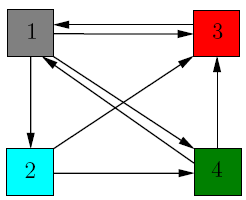
\includegraphics[width=\textwidth]{unweighted.png}
        \end{column}
        \begin{column}{0.5\textwidth}
            As a graph: Each website is represented by a node assigned with a PageRank value, denoted by PR(w). If a website w has a link to another website v (meaning there are an outbound link from w and an inbound link to v), then there is a directed edge from node w to node v. Multiple links from w to v is treated as a single edge from node w to v, and all self-links from a website to itself are ignored. Thus, this is a node-weighted, simple, no self-loop directed graph.
        \end{column}
    \end{columns}
\end{outline}
\end{frame}

\begin{frame}
\frametitle{Edge Weights}
\begin{columns}
    \begin{column}{0.5\textwidth}
        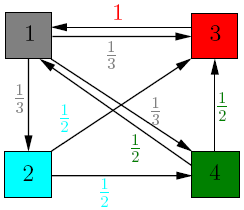
\includegraphics[width=\textwidth]{weighted.png}
    \end{column}
    \begin{column}{0.5\textwidth}
        This edge has its weight equal to PR(*w*) divided by the total number of outbound links of $w$, L($w$). Then recipient node $v$ "receives" the PageRank value of $w$, adding to its own value, i.e., PR($v$) += PR($w$)/L($w$). 
        
        In another words, for a given node in the graph:

        \textbf{An outbound link} will "give" away the PR value of the source node to the recipient node.  

        \textbf{An inbound link} will add the PR value from the source node to the recipient node.
    \end{column}
\end{columns}
\end{frame}

\begin{frame}[t]{Perspectives for Solving}
    \begin{itemize}
        \setlength\itemsep{1em}
        \item There are two ways to understand the problem:
        \item[1)] as an Eigenvector problem
        \item[2)] as a probability problem
        \item Both perspectives use linear algebra 
    \end{itemize}
\end{frame}

%\begin{frame}{Adjacency Matrix}
%\begin{columns}
%    \begin{column}{0.5\textwidth}
%        \centering
%        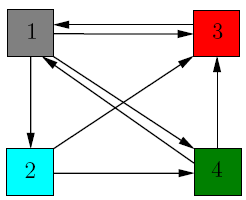
\includegraphics[width=\textwidth]{unweighted.png}
%    \end{column}
%    \begin{column}{0.5\textwidth}
%        \centering
%        {\Large$A = \begin{pmatrix}
%            0 & 1 & 1 & 1\\
%            0 & 0 & 1 & 1\\
%            1 & 0 & 0 & 0\\
%            1 & 0 & 1 & 0\\
%        \end{pmatrix}$}
%    \end{column}
%\end{columns}
%\begin{outline}
%    \1 No self loops means the main diagonal is all zeros
%\end{outline}
%\end{frame}

\begin{frame}[t]{Eigenvector Problem}

\end{frame}

\begin{frame}[t]{Probability Problem}

\end{frame}

\begin{frame}[t]{Power Iteration}

\end{frame}

\begin{frame}[t]{Spider Traps and Deadends}

\end{frame}

\begin{frame}[t]{Random Teleports + Damping factor}
    
\end{frame}


\section{Applications}
\begin{frame}[t]
    \frametitle{Applications}
    \begin{outline}
        \1 PageRank is perhaps the most famous search ranking algorithm. Googles high-quality search engine results are directly correlated to PageRank
        \1 There are a remarkable wide variety of applications of the PageRank algorithm that apply to non-search engine contexts.
        \1 Its simplicity and elegance allow PageRank to be a more general and powerful tool.
        \1 Let's look at the applications of PageRank and its connection to Twitter.

    \end{outline}
\end{frame}

\begin{frame}[t]
    \frametitle{Twitter}
    \begin{outline}
        \1 In 2010, Twitter was lagging behind and was lacking a user recommendation service. 
        \1 This was perceived both externally and internally as a critical gap in Twitter’s product offerings, so quickly launching a high-quality product was a top priority.
        \1 Twitter is unique because of the asymmetric nature of the following relationship—a user can receive messages from another without reciprocation. 
        \1 This differs substantially from other social networks such as Facebook or LinkedIn, where social ties can only be established with the consent of both participating members.
    \end{outline}
\end{frame}

\begin{frame}[t]
    \frametitle{Introducing PageRank}
    \begin{outline}
        \1 This works well with PageRank because we can determine outbound and inbound links.
        \1 A user $u$ is likely to follow those who are followed by users that are similar to $u$. 
        \1 These users are in turn similar to $u$ if they follow the same (or similar) users.
        \1 Therefore using Page Rank, Twitter is able to offer unique recommendations for users. 
        \1 By analyzing who the user follows and who those users follow, the PageRank algorithm will allow Twitter to make specific recommendations for each user. 
        \1 Essentially, the more outbound links that an account receives correlate to a higher PageRank score.        
    \end{outline}
\end{frame}

\end{document}